\begin{frame}{\large Multi-fix Rectification: Prior work}

% MFR 
% 
% Iterative incremental SAT 
% Verification: Computer Algebra
% [Lv. et al, TCAD’13] [Sayed. et al, DATE’16] [Ritirc. et al, FMCAD’17]
% Rectification using Craig Interpolants in Algebraic Geometry
% [Our research group, Gupta. et al, VLSI-SOC’18]
% Automated Debugging using Computer Algebra
% [Mishra. et al, ICCD’17] [Mishra. et al, DATE’16] [Ciesielski. et al, DAC’15]
%  Incorrect and incomplete: Approach fails on the above circuit
\bi
\item Craig interpolation and/or iterative SAT solving [{\it Huang. et al}, DAC'11][{\it Huang. et al}, DATE'12]
\bi
	\item Iteratively and incrementally patch the circuit
	\item Compute multiple partial single-fix functions at the given $m$ targets
\ei
\item Resource aware ECO patch generation [{\it Jiang. et al}, DAC'18][{\it Mishchenko. et al}, DAC'18]
		[{\it Fujita. et al}, ISCAS'19]
\item Approaches infeasible on arithmetic circuits
\item Symbolic sampling technique [{\it Jiang. et al}, DAC'19]
\bi
	\item Enumerate rectification points functionally and match the circuitry of patches implicitly
	\item Scalability achieved by modeling computations in symbolic sampling domain
	% \item Doesn't discuss application to arithmetic circuits
\ei
\ei
\end{frame}

% \begin{frame}{\large MFR Contribution: Approach on finite field circuits}
% % \item In a general setting a SFR may not exist even for trivial design bugs in smaller circuits.
% % \bi
% % 	\item Need an approach to address multi-fix rectification
% % \ei
% \bi
% 	\item Checks whether a given circuit $C$ can be rectified at given $m$ targets
% 	% \item Modeling the problem on the lines of SFR may be computationally expensive
% 	\item Word-level formulation
% 	\bi
% 		\item Interpret these $m$ targets as an $m$-bit vector word $W$
% 		\item Our approach aims to test for MFR in a single step
% 		% \item Obviates iterative correction tests, individually, at $m$ targets
% 		\item Multi-fix patch is computed at the bit-vector (word) level in terms of primary inputs: $W=U(X_{PI})$
% 		\bi
% 			\item Function mapping, $f_W:\F_2^n \rightarrow \Fkm$ 
% 			\item Synthesize individual patches from the word-level expression
% 		\ei
% 	\ei
% \ei
% \end{frame}

\begin{frame}{\large Application: Multi-fix Rectification}
\begin{figure}[hbt]
\centering
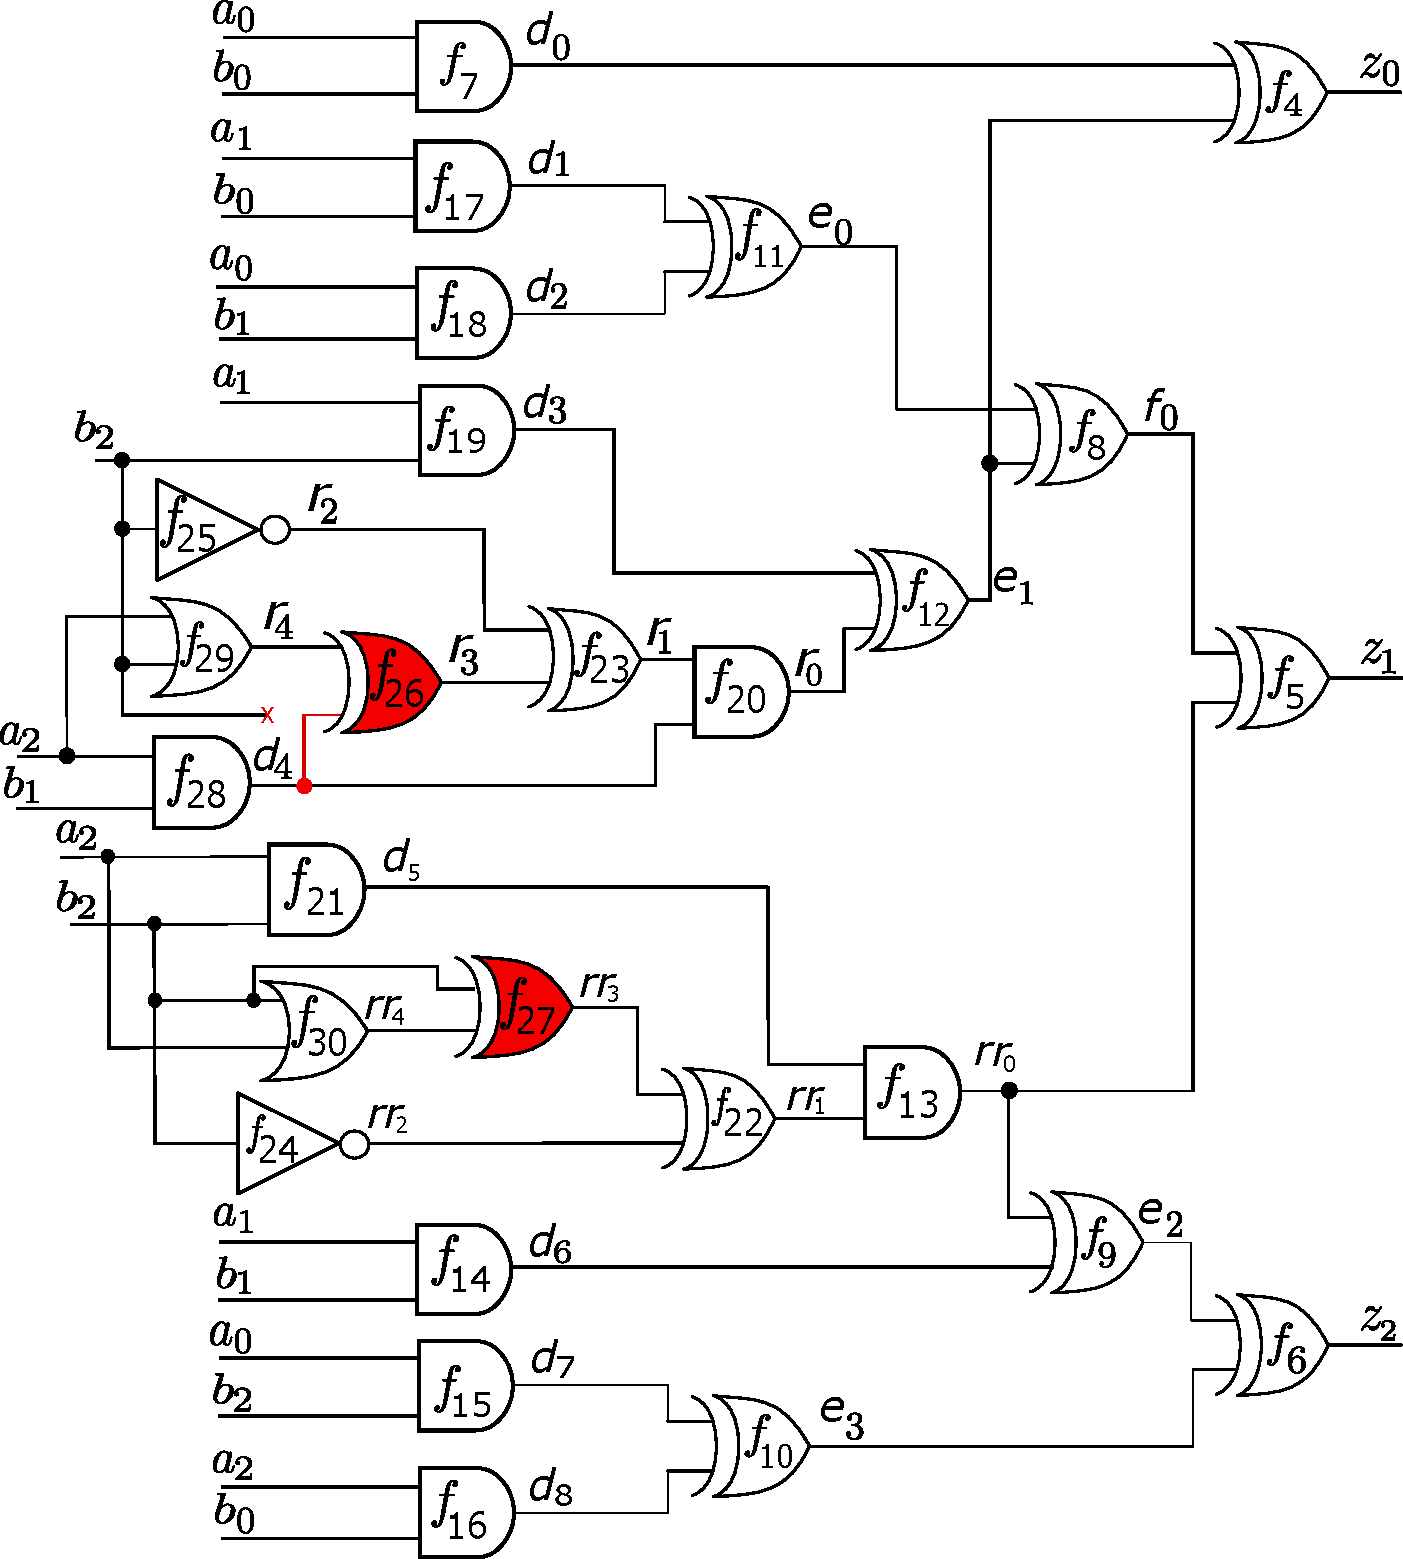
\includegraphics[scale=0.24]{mas_3_ddc_mfr_a.pdf}
\caption*{A faulty implementation of a 3-bit ($n$=3) Mastrovito multiplier
% ($n$=3) with gate replacement bugs introduced at nets $d_5$ (AND replaced with an OR) and $d_2$ (AND replaced with an XOR), and a wire replacement bug at net $e_0$ (input shorted to $d_0$ instead of $d_1$).
}
\end{figure}
\end{frame}

\begin{frame}{\large Application: Word-level representation}
\begin{figure}[hbt]
\centering
    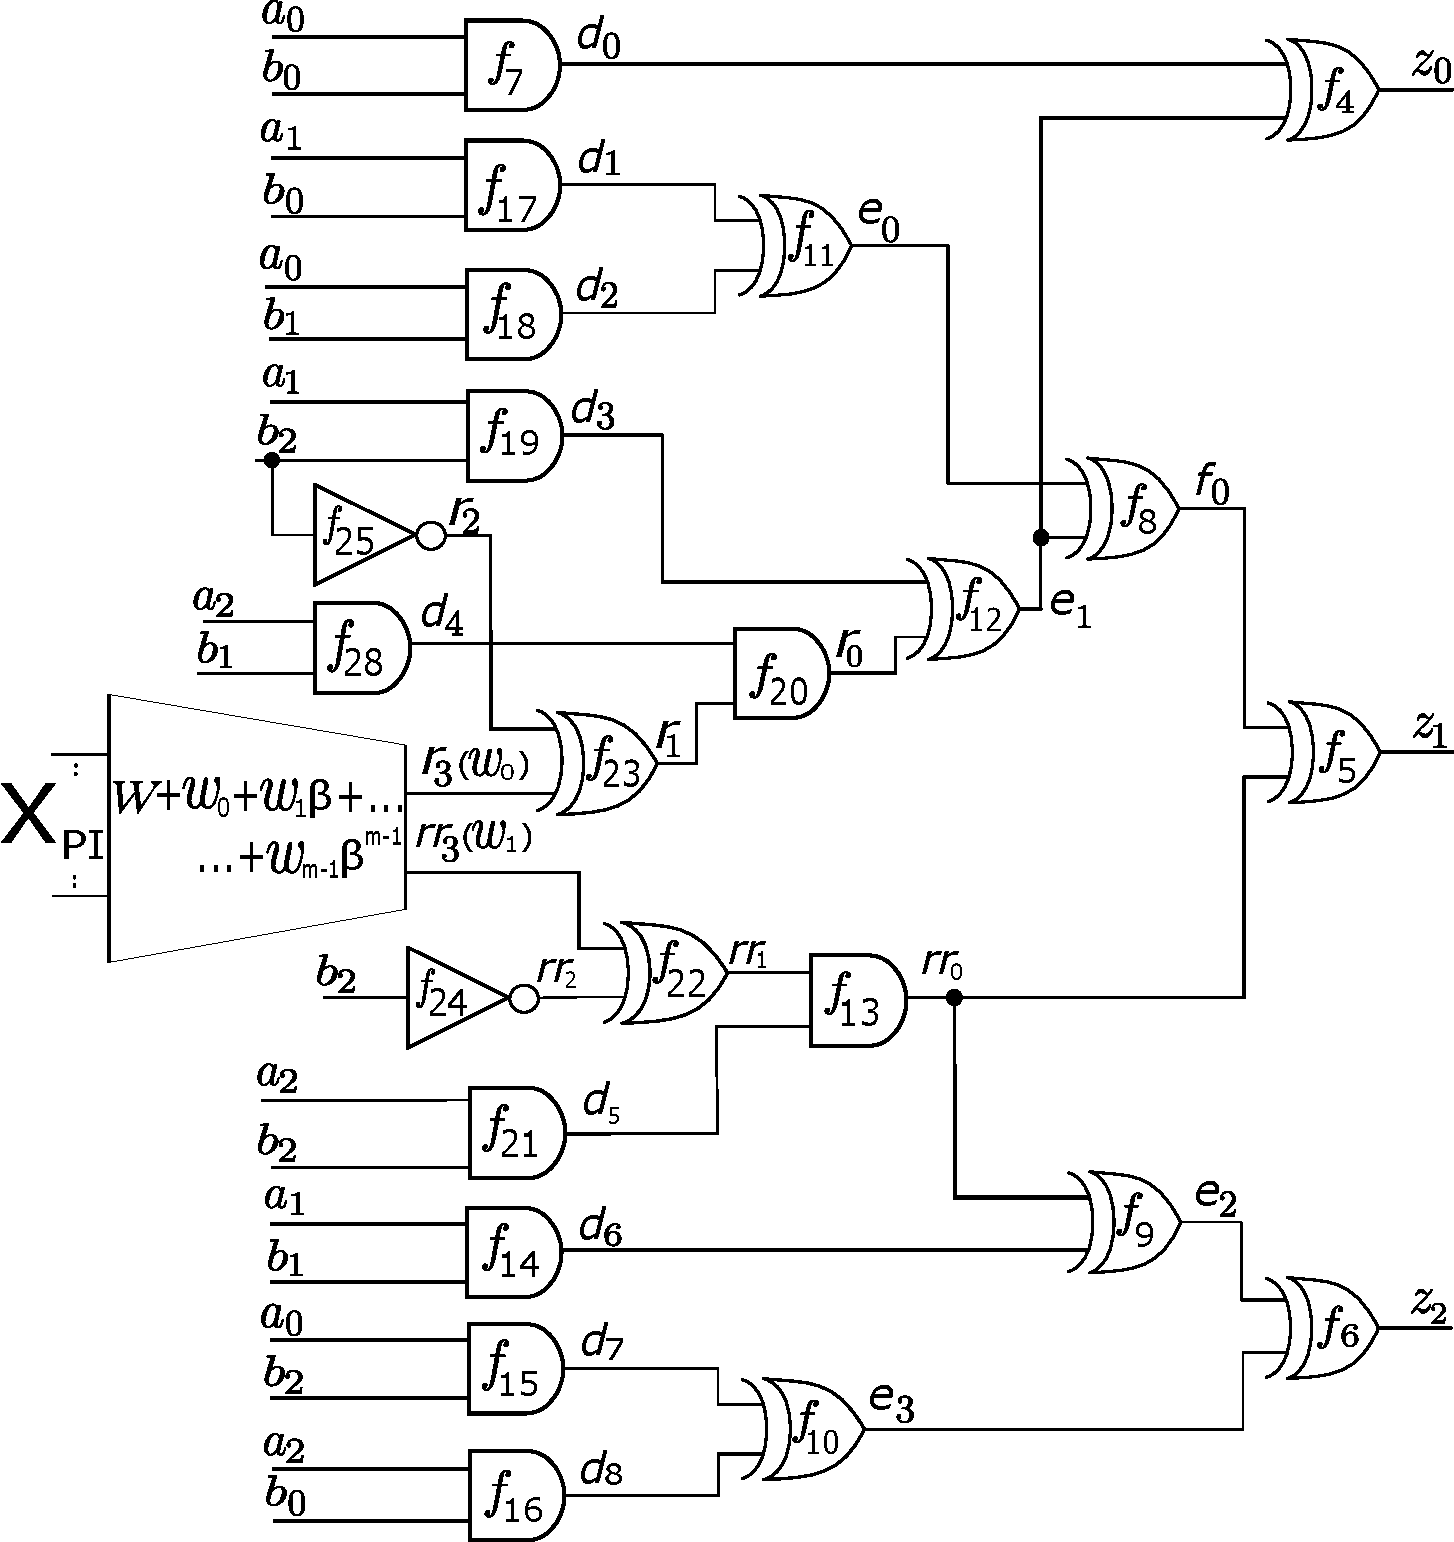
\includegraphics[scale = 0.24]{mas_3_ddc_mfr_b.pdf}
    \caption*{
    Patch function modeled as a 2-bit-vector word ($m$=2) $W=\{r_3,rr_3\} = r_3+\be\cdot rr_3$, ($w_0=r_3, w_1=rr_3$).}
    \label{fig:mas_bug_Wb}
\end{figure}
\end{frame}


\begin{frame}{\large MFR Notation: Field setup}
\bi
	\item Circuit with data-path size $n$ modeled over $\Fkn$
	\bi
		% \item Polynomials modeled over $R=\Fkn[Z,A,x_1,\dots,x_d]$
		% \bi
		% 	\item $\{x_1, \dots$ $, x_d\}$ are all the bit-level variables (nets) in the circuit
		% 	\item $Z$ and $A$ are the word-level output and input, respectively
		% \ei
		\item $\Fkn$ is constructed as $\Fkn = \Ftwo[x]\pmod{P_n(x)}$
		\bi
			\item $P_n(x) \in \F_2[x]$ is a given degree-$n$ primitive polynomial; $P_n(\ga) =0$ 
			% [$\ga$ as one of its root].
		\ei
		\item  The word-level polynomials for $Z,A$ are modeled as:
		\bi
			\item $f_Z: Z + \sum_{i=0}^{n-1}\ga^iz_i,~f_A: A + \sum_{i=0}^{n-1}\ga^ia_i$ 
		\ei
	\ei 
	\vspace{0.1in}
	\vspace{0.1in}
	\item Patch size $m$ modeled over $\Fkm$
	\bi
		\item $\Fkm$ is constructed as $\Fkm = \Ftwo[x]\pmod{P_m(x)}$
		\bi
			\item We select a degree-$m$ primitive polynomial $P_m(x)\in \F_2[x]$; $P_m(\be) =0$ 
			% [$\be$ as one of its root].
		\ei
		\item  The word-level polynomial for $W$ is modeled as:
		\bi
			\item $f_w: W + \sum_{i=0}^{m-1}\be^iw_i$
			\item $\{w_0,\dots,w_{m-1}\} \subset \{x_1,\dots,x_d\}$
		\ei
	\ei
\ei
\end{frame}

% \begin{frame}{\large Mathematical Challenge: Picking $P_k(x)$}
% \bi 

% 	\item Need to represent and manipulate circuit polynomials and the patch function polynomials in one unified domain (composite field)
% 	% \bi
% 	% 	\item How to relate algebraic numbers of lower field to algebraic numbers of higher fields?
% 	% \ei
% 	\vspace{0.1in}
% 	\item Selecting arbitrary $P_k(x)$ leads to erroneous results 
% 	\vspace{0.1in}
% 	\item Solved using Univariate Polynomial Factorization

% \ei
% \end{frame}

\begin{frame}{\large MFR Challenges: $\Fkk$ and $P_k(x)$}
\bi
	% \item Determine the smallest single field ($\Fkk$) to operate both circuit ($\Fkn$) and patch ($\Fkm$)
	% \vspace{0.1in}
	\item Smallest $k$ is $LCM(n,m)$
	\bi
		\item $\Fkk \supset \Fkn$ and $\Fkk \supset \Fkm$
		\item $\Fkk$ is constructed as $\Fkk = \Ftwo[x]\pmod{P_k(x)}$
		\bi
			\item $P_k(x)$ is a degree-$k$ primitive polynomial; $P_k(\al) =0$ 
		\ei
	\ei
	\vspace{0.1in}
	\item  Mathematical challenge: Given $P_n(x)$ and $P_m(x)$, compute $P_k(x)$ such that
	$P_n(\ga)= P_m(\be)=P_k(\al)=0$
	\vspace{0.1in}
	\bi
		\item $\ga = \al^{(2^k-1)/(2^n-1)} = \al^{\lambda}$
		\item $\be = \al^{(2^k-1)/(2^m-1)} = \al^{\mu}$
	\ei
	\vspace{0.1in}
	\item Solved using factorization of univariate polynomials over finite fields
\ei

\end{frame}

% \begin{frame}{\large MFR Notations: Univariate Polynomial factorization (UPF) }
% \bi
% 	\item Given a monic univariate polynomial $f \in \F_q[X]$, where $\F_q$ is any finite field
% 	\vspace{0.1in}
% 	\bi 
% 		\item Find a complete factorization $f = f_1^{e_1}\cdot f_2^{e_2}\cdots f_l^{e_l}$ 
% 		\bi
% 			\item Where $f_1, f_2,\dots, f_l$ are pairwise distinct monic 
% 			irreducible polynomials in $\F_q[X]$ and $e_1,\dots,e_l$ are positive integers.
% 		\ei
% 	\ei
% 	\vspace{0.1in}
% 	% \item We employ existing implementation of UPF from computer algebra tool {\it SINGULAR} 
% \ei
% \end{frame}

\begin{frame}{\large Contribution: Computing $P_k(x)$}
\bi
	\item Obtain UPFs of $P_n(x^{\lambda})$ and $P_m(x^{\mu})$ in $\F_2[x]$
	% \bi
	% 	\item Coefficients will be in $\Ftwo$ and degrees will be less than $\lambda$ and $\mu$, respectively.
	% 	\bi
	% 		\item $P_n(x^{\lambda})=P_{n1}^{a1}\cdot P_{n2}^{a2}\cdots P_{nl}^{al}$, and 
	% 		\item $P_m(x^{\mu}) = P_{m1}^{b1}\cdot P_{m2}^{b2}\cdots P_{mg}^{bg}$
	% 	\ei
	% \ei
	\vspace{0.1in}
	\item Then, $\exists P_{k}(x) \in \F_2[x]$ as a common factor of $P_n(x^{\lambda})$ and $P_m(x^{\mu})$, such that:
	\bi
		\item $P_{k}(x)$ is a degree-$k$ primitive polynomial in $\F_2[x]$ with $P_k(\al)=0$
	\ei
\ei
\end{frame}

\begin{frame}{\large Application: Word-level representation}
\begin{figure}[hbt]
\centering
    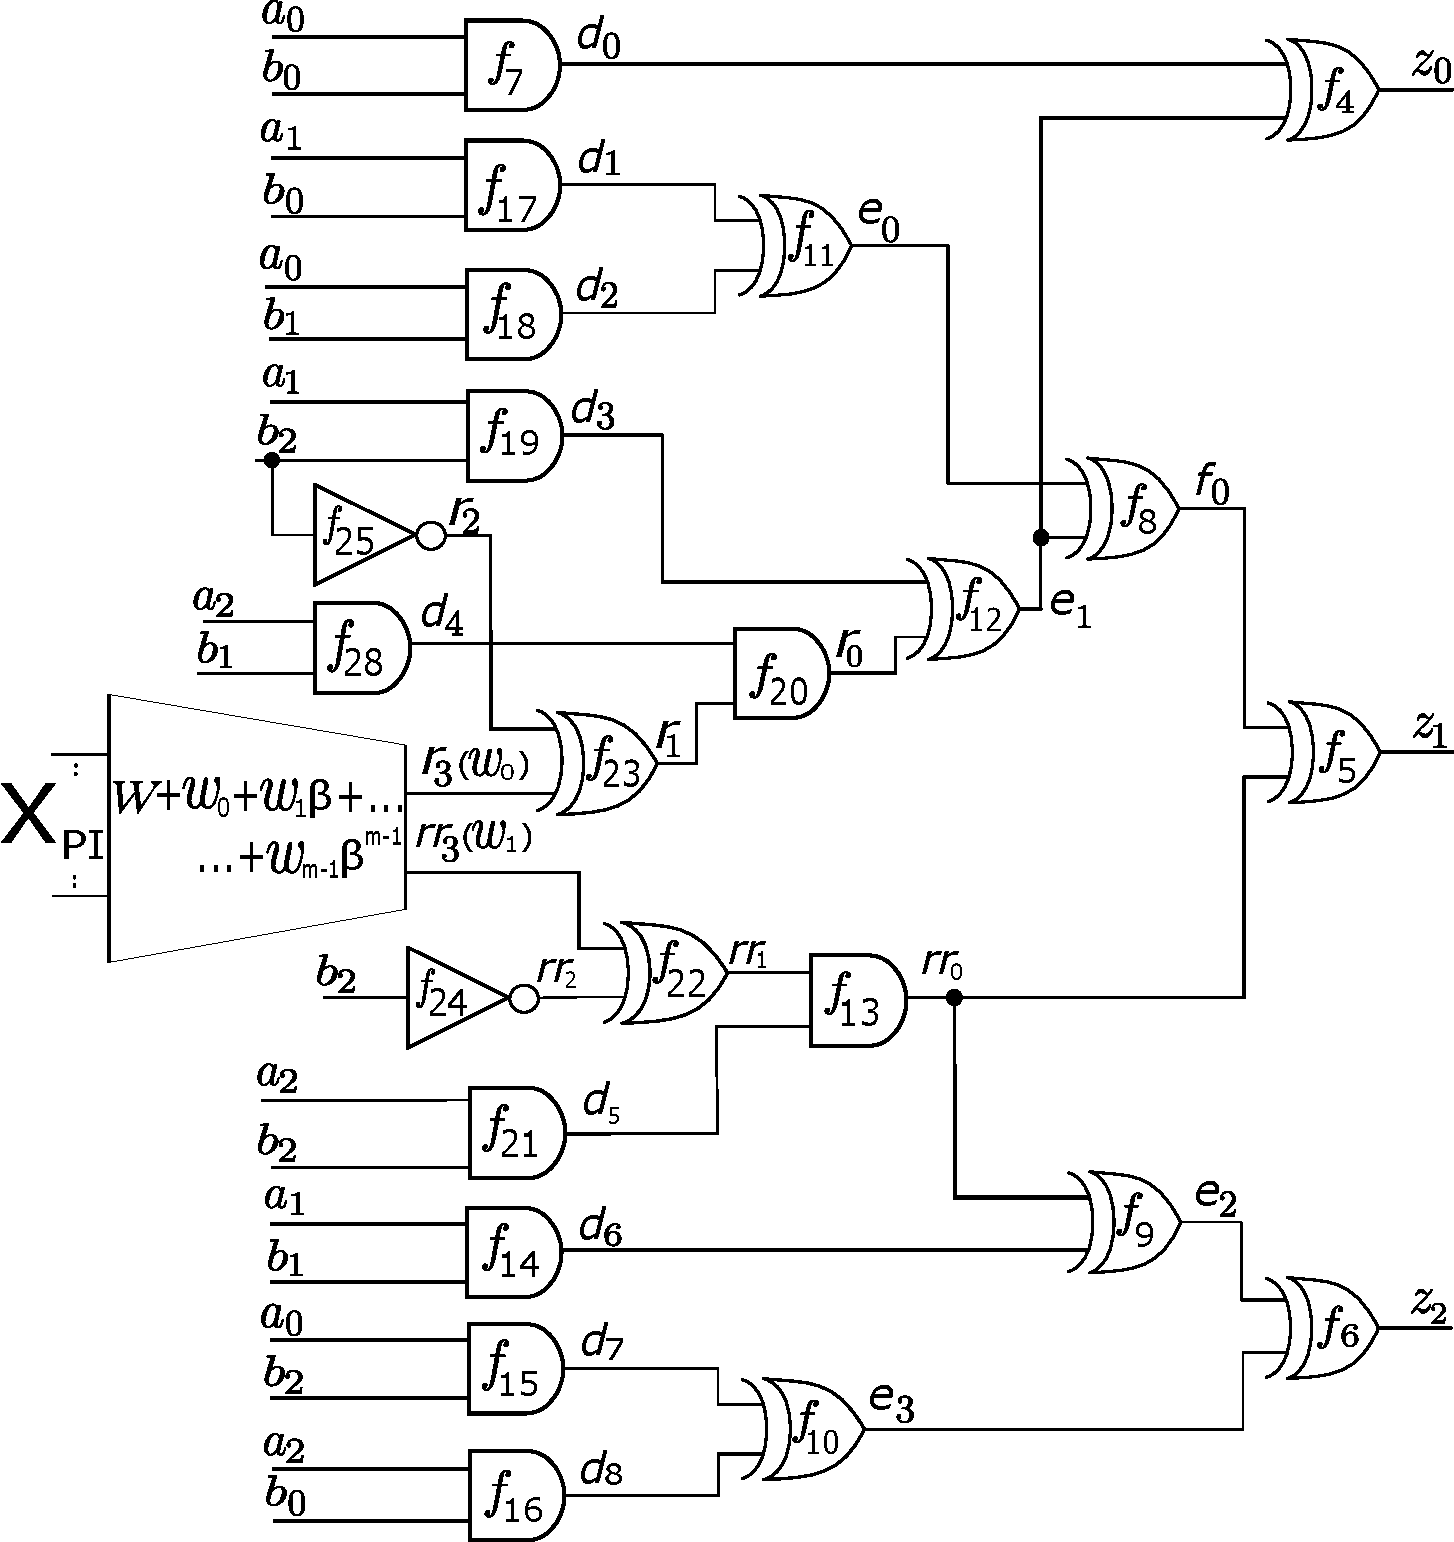
\includegraphics[scale = 0.24]{mas_3_ddc_mfr_b.pdf}
    \caption*{
    Patch function modeled as a 2-bit-vector word ($m$=2) $W=\{r_3,rr_3\} = r_3+\be\cdot rr_3$, ($w_0=r_3, w_1=rr_3$).}
    \label{fig:mas_bug_Wb}
\end{figure}
\end{frame}

\begin{frame}{\large Application: Computing $P_k(x)$}
\bi
\item $P_3(x) = x^3+x+1,~~P_2(x) = x^2+x+1,~~\ga = al^9,~~\be=\alpha^{21}$

\vspace{0.1in}
	\item Composite field: $k=LCM(2,3)=6$
	\vspace{0.1in}
	\bi
		\item $ UPF(P_3(x^9)) = (x^9)^3+(x^9)+1 =
  (x^6+x^5+x^2+x+1)(x^6+x^5+1)(x^6+x^4+x^3+x+1)(x^6+x^4+x^2+x+1)(x^3+x+1);$
		\vspace{0.1in}
		\item $UPF(P_2(x^{21})) = (x^{21})^2+(x^{21})+1 =
  (x^6+x^5+x^2+x+1)(x^6+x^5+1)(x^6+x^4+x^3+x+1)(x^6+x^5+x^3+x^2+1)
  (x^6+x^5+x^4+x+1)(x^6+x+1)(x^6+x^3+1);$
		\vspace{0.1in}
		\item We choose $P_6(x)=x^6+x^5+1$ as the required $P_k(x)$.
	\ei
\ei
\end{frame}

\begin{frame}{\large MFR Notation: Incorrect $P_k(x)$}
\bi
	\item Note that if we incorrectly choose $P_k(x)=x^6+x^3+1$
	\item For its root $\al$, we have
	\begin{align*}
\alpha^6 + \alpha^3 + 1 &= 0\\
 (\alpha^3)(\alpha^6 +\alpha^3 + 1) &= 0 ~(\text{multiply by}~\alpha^3)\\
\alpha^9 + \alpha^6 + \alpha^3 &= 0 \\
 \gamma + 1 &= 0
\stepcounter{equation}\tag{\theequation}\label{ll} 
\end{align*}
	\item However, $\ga \neq 1$, as $\ga$ is a primitive element of $\Fkn$
	\item Selecting arbitrary $P_k(x)$ leads to erroneous results
\ei
\end{frame}


\begin{frame}{\large MFR Notation: Word-level Formulation steps}
\bi
	\item Modify field to $\Fkk$ and compute $P_k(x)$
	\item Update ring by adding word-level target representation $W$ 
	\vspace{0.1in}
	\item Construct a polynomial set $F'$ as follows:
	\bi
		\item Start with $F' = F$
		\item Remove polynomials with $w_i$'s as leading terms
		\item Substitute for $w_i$'s the respective word-level polynomials
		\item Add $f_w: W + \sum_{i=0}^{m-1}\be^iw_i$
	\ei

\ei
\end{frame}

\begin{frame}{\large MFR Application: Word-level Formulation }
\bi
	\item 2-bit rectification patch over the 3-bit circuit can be performed over the field $\F_{2^6}$
	\bi
		\item Field $\F_{2^6} = \F_2[X]$ (mod $P_6(X)$)
	\ei
	\vspace{0.1in}
	\item Update polynomial set $F$ to $F'$ as:
	\begin{center}
		\begin{align*}
			F'=\{f_1,\dots,f_3,f'_4,f'_5,f_6,f'_7,f'_8,f_9,f_w,f_{11},f_{13}\dots,f_{20}\}
		\end{align*}
		{\small\begin{flalign*}
			f'_4:z_0 + (\be W^2 +\be^2 W) + d_0;     &\quad f'_5:z_1 + f_0 + (W^2+W); \\
			f'_7:f_0 + (\be W^2 +\be^2 W) + e_1;   &\quad f'_8:e_2 + (W^2+W) + d_6; \\
			f_w:W + e_0 + \be d_5;             &\quad \be=\al^{21} ; \ga=\al^9;
		\end{flalign*}}
	\end{center}

\ei
\end{frame}

\begin{frame}{\large MFR Contribution: Rectification Check}
%ATPG V() V() = empty
%we have an algebraic proof which is there in the proposal
\bi
	\item Multi-fix rectification at target $W$
	\vspace{0.1in}
	\bi
		\item Construct the following ideals:
		\bi
			\item {\small $J_i = \langle F'_i\rangle =\{f'_1,\dots,f_w=W+\delta(i),\dots,f'_s\}$}
				:$1 \leq i \leq 2^m$, $\delta(0)=0, \delta(1)=1,\delta(2)=\be,\dots,\delta(2^m)= \be^{2^m-2}$
		\ei
		\vspace{0.1in}
		\item Performing the reductions for all $1 \leq i \leq 2^m$: 
		\bi
			\item $f\xrightarrow{F'_i, F_0}_+r_i $
		\ei
		\item Let $V_{\Fq}(r_i)$ denote the varieties of the respective $r_i$'s
		\vspace{0.1in}
		\item Multi-fix rectification exists at target $W$: \\ \\ 
				\centering
				{\bf if and only if} $\bigcup\limits_{i=1}^{2^m}V_{\Fq}(r_i) = \Fq^{|X_{PI}|} = V(J_0)$
	\ei
\ei
\end{frame}

\begin{frame}{\large MFR Application: Rectification Check}
\bi
	\item Constructing the $J_i$ ideals:
	\bi
		\item {\small$J_1 = \langle F'_1\rangle$, where $F'_1[f_w]=W+\delta(1)=W$},
		\item {\small$J_2 = \langle F'_2\rangle$, where $F'_2[f_w]=W+\delta(2)=W+1$},
		\item {\small$J_3 = \langle F'_3\rangle$, where $F'_3[f_w]=W+\delta(3)=W+\be$},
		\item {\small$J_4 = \langle F'_4\rangle$, where $F'_4[f_w]=W+\delta(4)=W+\be^2$}
	\ei
	\vspace{0.1in}
	\item Reducing the specification $f: Z+A\cdot B$ modulo these ideals, we get:
\bi
\item $rem_1 = f \xrightarrow[]{F'_1\cup F'_{0}}_+{\al^{27} (a_2b_1b_2)+\al^{36} (a_2b_2)}$
\item $rem_2 = f \xrightarrow[]{F'_2\cup F'_{0}}_+{\al^{27} (a_2b_1b_2+a_2b_1)+\al^{36} (a_2b_2)}$
\item $rem_3 = f \xrightarrow[]{F'_3\cup F'_{0}}_+{\al^{27} (a_2b_1b_2)}$
\item $rem_4 = f \xrightarrow[]{F'_4\cup F'_{0}}_+{\al^{27} (a_2b_1b_2+a_2b_1)}$
\ei
	\item Compute $GB(r_1\cdot r_2 \cdot r_3 \cdot r_4, F_0)=F_0$
	\item Target $W$ with nets $r_3$ and $rr_3$ admits MFR
\ei
\end{frame}

\begin{frame}{\large Future work: Rectification function}

\bi
\item A polynomial which can be computed to rectify the circuit
	\bi
		\item $W = a_2b_1b_2 + \beta \cdot a_2b_2$
		\item $r_3 = (a_2 \wedge b_1 \wedge b_2),~~rr_3 = (a_2 \wedge b_2)$
	\ei
\ei

\end{frame}

% \begin{frame}{\large MFR Pseudocode}
% \begin{figure}[hbt]
% \centering
%     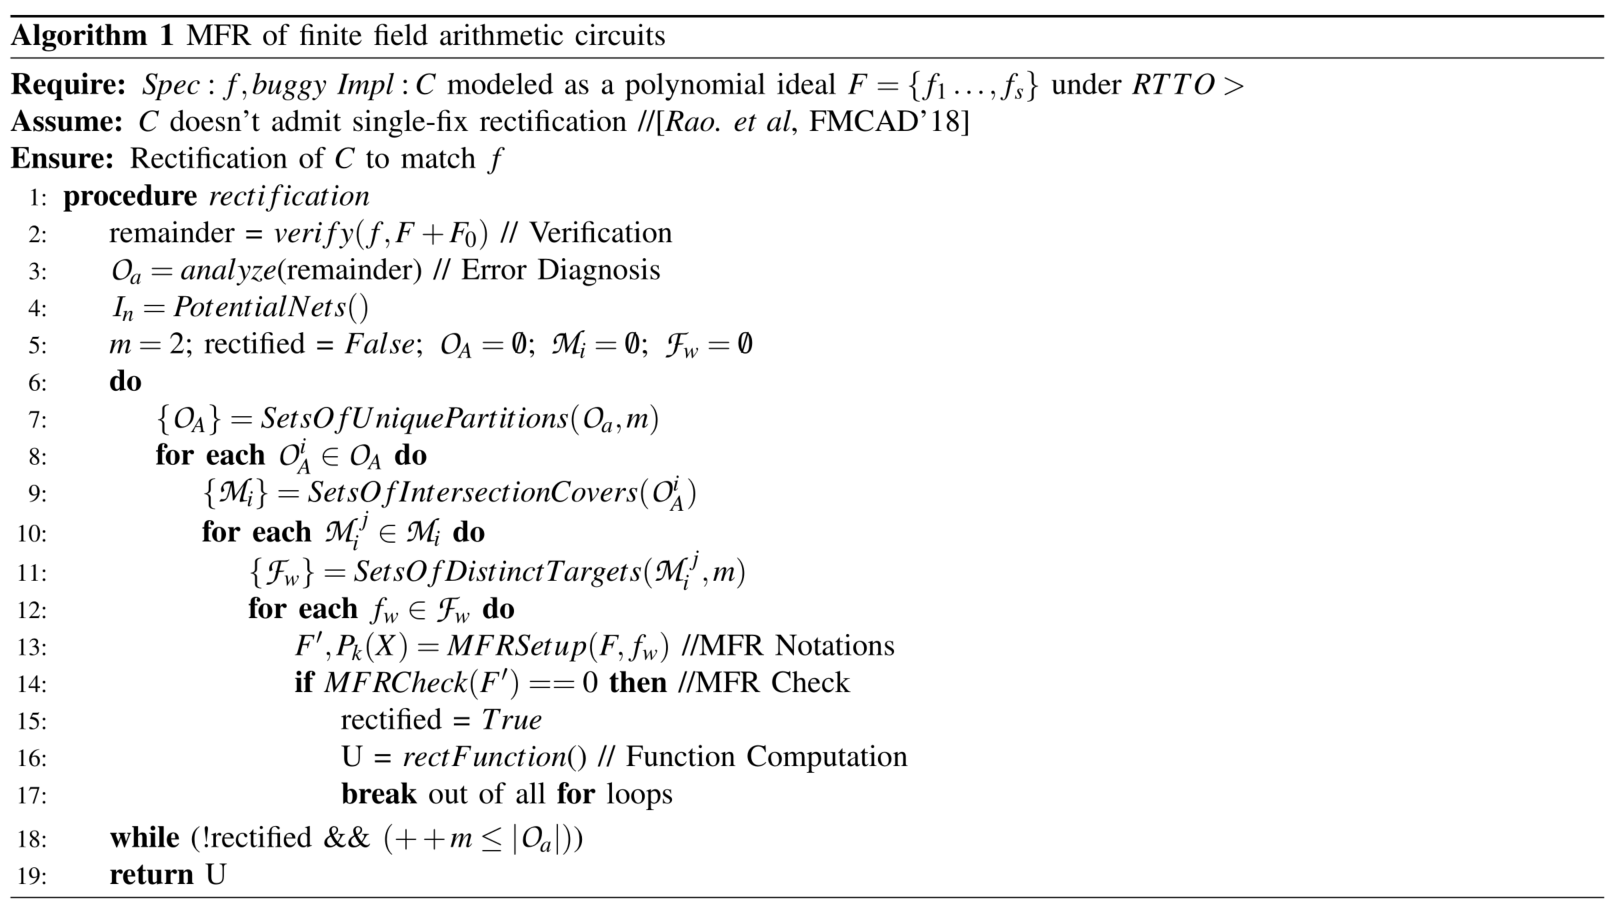
\includegraphics[scale = 0.43]{algo.png}
% \end{figure}
% \end{frame}

% \begin{frame}{\large Research Objective: Synthesis of Rectification Function}
% \begin{figure}[hbt]
%     \begin{center}
%     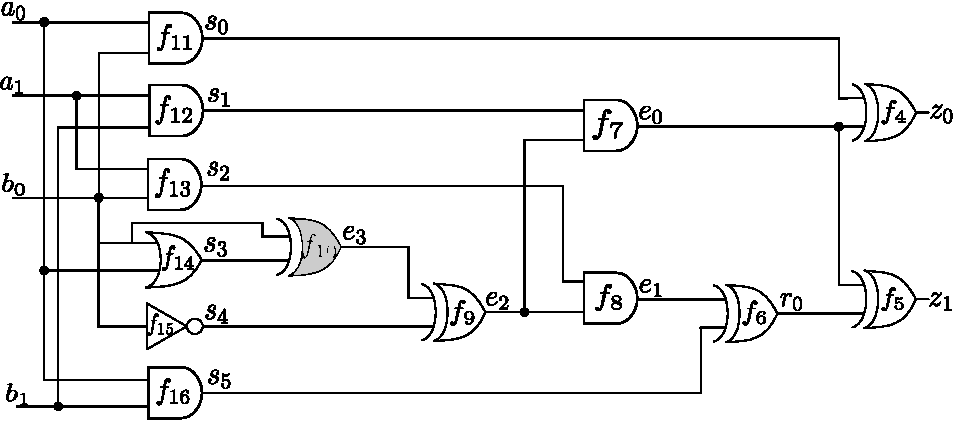
\includegraphics[scale = 0.7]{mas_red_bug-eps-converted-to.pdf}
%     \end{center}
% %    \vspace{-4ex}
%     \caption*{\small A 2-bit buggy modulo
%       multiplier implementation. 
%     %   with the bug at
%     % net $e_3$. A correct implementation will have an AND gate at $e_3$,
%     % which has been replaced by an XOR gate.
%     }
%     \label{fig:mas_both}
% \end{figure}
% \end{frame}

% \begin{frame}{\large Research Objective: Exploring don't cares}
% \begin{small}
% $r \in \langle h_{10},f_{11},f_{12},f_{13},f_{14},f_{15},f_{16}\rangle
%   + \langle F_{0}^{PI}\rangle$ \\
% $r = U\cdot h_{10} + h_{11}f_{11} + h_{12}f_{12}+h_{13}f_{13}+h_{14}f_{14}+h_{15}f_{15}+h_{16}f_{16}$ \\
% $U = b_0$; $U^1 = a_1*b_0$; $U^2 = a_1*b_1*b_0+a_1*b_1+a_1$;
% \end{small}
% {\tiny 
% \begin{table}[ht]
%     \centering
%     \begin{tabular}{|c|c|c|c|c|} \hline
%       $\{a_0a_1b_0b_1\}$ & $h_{10}$ & $U$ & ${U^1}$ & ${U^2}$ \\ \hline
% 		0000 & 0     & 0 & 0 & 0 \\ \hline
% 		0001 & 0     & 0 & 0 & 0 \\ \hline
% 		0010 & 0     & 1 & 0 & 0 \\ \hline
% 		0011 & 0     & 1 & 0 & 0 \\ \hline
% 		0100 & 0     & 0 & 0 & 1 \\ \hline
% {\it    0101}& (x+1) & 0 & 0 & 0 \\ \hline
% {\bf    0110}& (x)   & 1 & 1 & 1 \\ \hline
% {\bf	0111}& 1     & 1 & 1 & 1 \\ \hline
% 		1000 & 0     & 0 & 0 & 0 \\ \hline
% 		1001 & 0     & 0 & 0 & 0 \\ \hline
% 		1010 & 0     & 1 & 0 & 0 \\ \hline
% 		1011 & 0     & 1 & 0 & 0 \\ \hline
% 		1100 & 0     & 0 & 0 & 1 \\ \hline
% {\it    1101}& (x+1) & 0 & 0 & 0 \\ \hline
% {\bf    1110}& (x)   & 1 & 1 & 1 \\ \hline
% {\bf    1111}& 1     & 1 & 1 & 1 \\ \hline
%     \end{tabular}
%     \caption{Evaluating quotient and rectification solutions}
% \end{table}}

% \bi
% 	\item Challenge: Word-level formulation of don't cares
% \ei

% \end{frame}

% \begin{frame}{\large Research Objective: Logic optimization using don't cares}
% \bi
% 	\item $h_{10}$ represents the ODCs for the selected target $e_3$
% 	\bi
% 		\item Algorithm to explore don't care setup
% 	\ei
% 	\vspace{0.1in}
% 	\item Logic simplification using permissible functions
% 	\bi
% 		\item {\it Fujita} has an approach using BDDs
% 		\item Investigate the application in algebraic setting
% 	\ei
% \ei
% \end{frame}

